%\documentclass[a4paper,11pt]{article}
\documentclass[final,3p,times,twocolumn]{elsarticle}
\pdfoutput=1 % if your are submitting a pdflatex (i.e. if you have
             % images in pdf, png or jpg format)

%\usepackage{elsarticle} % for details on the use of the package, please
                     % see the JINST-author-manual

\usepackage[utf8]{inputenc}
\usepackage{textcomp}
\usepackage{lineno}
\usepackage{color}
\newcommand{\todo}[1]{\textcolor{red}{{#1}}}
\usepackage[outdir=./]{epstopdf}
\usepackage{upgreek}
\usepackage{amsmath}
\usepackage{subcaption}
\usepackage{hyperref}
\hyphenation{time-stamped}
%\title{\boldmath Commissioning and performance in beam tests of the highly granular SiW-ECAL technological prototype for the ILC}

% e-mail addresses: only for the forresponding author
%\ead{irles@lal.in2p3.fr}
%\collaboration[]{on behalf of the CALICE collaboration}

\begin{document}

\begin{frontmatter}
  \title{Beam test performance of the highly granular SiW-ECAL technological prototype for the ILC.}

  % \ead{irles@lal.in2p3.fr}

  \author[kyushu]{K.\,Kawagoe}
  \author[kyushu]{Y.\,Miura}
  \author[kyushu]{I.\,Sekiya}
  \author[kyushu]{T.\,Suehara}
  \author[kyushu]{T.\,Yoshioka}
  
  \author[lal]{S.\,Bilokin\corref{cor_iphc}}
  \author[lal]{J.\,Bonis}
  \author[lal]{P.\,Cornebise}
  \author[lal]{A.\,Gallas}
  \author[lal]{\underline{A.\,Irles}\corref{cor1}}
  \ead{irles@lal.in2p3.fr}
  \author[lal]{R.\,P\"oschl}
  \author[lal]{F.\,Richard}
  \author[lal]{A.\,Thiebault}
  \author[lal]{D.\,Zerwas}

  \author[llr]{M.\,Anduze}
  \author[llr]{V.\,Balagura}
  \author[llr]{V.\,Boudry}
  \author[llr]{J-C.\,Brient}
  \author[llr]{E.\,Edy}
  \author[llr]{G.\,Fayolle}
  \author[llr]{M.\,Frotin}
  \author[llr]{F.\,Gastaldi}
  \author[llr]{R.\,Guillaumat}
  \author[llr]{A.\,Lobanov}
  \author[llr]{M.\,Louzir}
  \author[llr]{F.\,Magniette}
  \author[llr]{J.\,Nanni}
  \author[llr]{M.\,Rubio-Roy\corref{cor_iphc}}
  \author[llr]{K.\,Shpak}
  \author[llr]{H.\,Videau}
  \author[llr,ihep]{D.\,Yu}

  \author[omega]{S.\,Callier}
  \author[omega]{F.\,Dulucq}
  \author[omega]{Ch.\,de la Taille}
  \author[omega]{N.\,Seguin-Moreau}

  \author[lpnhe]{J.E.\,Augustin}
  \author[lpnhe]{R.\,Cornat}
  \author[lpnhe]{J.\,David}
  \author[lpnhe]{P.\,Ghislain}
  \author[lpnhe]{D.\,Lacour}
  \author[lpnhe]{L.\,Lavergne\corref{cor_iphc}}
  \author[lpnhe]{J.M.\, Parraud}

  \author[skku]{J.\,S.\,Chai}
  
  \author[kek]{D.\,Jeans}


  %%%%
  \address[kyushu]{Department of Physics and Research Center for Advanced Particle Physics, 
      Kyushu University, 744 Motooka, Nishi-ku, Fukuoka 819-0395, Japan }

  \address[lal]{Laboratoire de l'Acc\'elerateur Lin\'eaire (LAL), CNRS/IN2P3 et
      Universit\'e de Paris-Sud XI, Centre Scientifique d'Orsay B\^atiment 200, BP 34, F-91898 Orsay 
    CEDEX, France}

  \address[llr]{Laboratoire Leprince-Ringuet (LLR)
    -- \'{E}cole polytechnique, CNRS/IN2P3, F-91128 Palaiseau Cedex, France }
  \address[ihep]{Institute of High Energy Physics of Beijing (IHEP), 19 Yuquan Rd, Shijingshan Qu, Beijing Shi, China}

  \address[omega]{Laboratoire OMEGA -- \'{E}cole polytechnique-CNRS/IN2P3, F-91128 Palaiseau Cedex, France}

  \address[lpnhe]{Laboratoire de Physique Nucl\'eaire et de Hautes Energies 
    (LPNHE), Universit\'e Sorbonne, UPD, CNRS/IN2P3, 4 Place Jussieu, 75005 Paris, France }
  
  \address[skku]{Department of Electrical and Computer Engineering, Sungkyunkwan Universtity, 16419, Suwon, Gyeonggi-do, Korea}
  \address[kek]{Institute of Particle and Nuclear Studies, KEK, 1-1 Oho, Tsukuba, Ibaraki 305-0801, Japan }

  \cortext[cor_iphc]{S.\,Bilokin is now at IPHC CNRS/IN2P3 from Strasbourg (France);  M.\,Rubio-Roy is now at SPINTEC CNRS from Grenoble (France); and L.\,Lavergne is now at IRAP from Toulouse (France)}
  \cortext[cor1]{Corresponding author}


\begin{keyword}
  Calorimeter methods, calorimeters, Si and pad detectors
\end{keyword}

%\maketitle
%\flushbottom


\begin{abstract}
The technological  prototype of the CALICE highly granular silicon-tungsten electromagnetic 
calorimeter (SiW-ECAL) has been tested in beam at DESY in 2017. 
In this test the setup comprised seven layers of 1024 channels and a size of $18\times18$ cm$^2$ each.
This article presents key performance results in terms of signal over noise ratios at different levels of the readout chain 
and a study of the uniformity of the detector response.   
\end{abstract}

\end{frontmatter}

\linenumbers


\section{Introduction}

The International Linear Collider, ILC \cite{Behnke:2013xla,Baer:2013cma,Adolphsen:2013jya,Adolphsen:2013kya,Behnke:2013lya},
is a next generation of $e^{+}e^{-}$
linear colliders project. It will
provide collisions of polarized beams with center-of-mass energies between 250 GeV and 1 TeV.
These collisions will be studied by multipurpose detectors.
The two proposed projects~\cite{Behnke:2013lya} --  the International
Large Detector (ILD) and the Silicon Detector
(SiD) -- are designed for the use of Particle Flow (PF) technique  \cite{Brient:2002gh,Morgunov:2004ed}, for the
reconstruction of the final state particles.
The PF techniques rely on single particle separation
to allow for the selection of the best information available
in the full detector to determine the final states of the collisions.
They allow reducing the impact of the poor resolution of the calorimeter systems
(compared with trackers) in the overall reconstruction
but require detectors with highly granular, compact
and hermetic calorimetric systems. Furthermore, the PF capabilities are enhanced when the calorimeters
are placed inside a large magnetic field that favours the separation of charged particles. 
This in turn calls for a compact design of the calorimeters.
Most of the R\&D efforts of such calorimeters 
for future linear colliders are carried out by the CALICE collaboration.

This document reports on the performance 
in beam test of the technological prototype of the silicon-tungsten electromagnetic calorimeter,
the SiW-ECAL.
The SiW-ECAL is the baseline choice for the ILD ECAL. It will be placed, together with the hadronic calorimeter
of the ILD, inside a magnetic field of at least 3T.
Silicon constitutes the active and tungsten the passive material of the detector. 
The overall thickness is 24 radiation
lengths ($X_{0}$) or about 1 interaction length.
The choice of silicon and tungsten makes possible the design
of a very compact calorimeter with high granularity in 3 dimensions. The baseline design
for the ILD foresees 26-30 layers in the barrel region enclosed in about 23 cm thick structures.
The active sensors will be segmented in squared cells of $5\times5$ mm$^2$,
for a total of $\sim$80 million readout channels for the barrel region of the ECAL of the ILD.
The dynamic range in each channel will range from 0.5 to 3000 MIPs, where the MIP acronym stands 
for both the most probable value of the energy deposited by a minimum-ionizing-particle and the particle itself.
In order to minimize external services and maximize the hermeticity, the very-front-end (VFE) electronics
must be embedded in the calorimeter modules and be cooled only passively.
In turn, to reduce overall power consumption, the SiW-ECAL will exploit the particular bunch structure
foreseen for the ILC: the $e^{+}e^{-}$ bunchs trains will arrive within
time windows of $\sim$1-2 ms width separated by $\sim200$ ms.
The data acquisition will be gated during these 1-2 ms and
the bias currents of the electronics will be shut down to save power during the idle time.
This technique is usually denominated as power pulsing. Finally,
the calorimeters will operate in self-trigger mode (each channel featuring a discriminator for internal trigger decision) and on-chip zero suppression mode. 

\section{The SiW-ECAL technological prototype}

The first SiW-ECAL prototype was the so-called SiW-ECAL physics prototype \cite{Anduze:2008hq}.
It was extensively tested at DESY, FNAL and CERN~\cite{Adloff:2011ha,Adloff:2008aa,Adloff:2010xj,CALICE:2011aa,Bilki:2014uep}.
The VFE was placed outside the active area with no particular constraints on power consumption.
It consisted of 30 layers of silicon sensors alternated with tungsten plates 
yielding a total of 24 $X_{0}$.
The active layers were made of a matrix of $3\times3$ silicon sensors of 500 $\upmu$m thickness. Each of these sensors was segmented in matrices of
$6\times6$ squared pixels of $10\times10$ mm$^2$.

The new generation prototype dubbed the SiW-ECAL technological prototype addresses the main technological challenges: compactness,
power consumption reduction through power pulsing and VFE inside the detector.

\begin{figure*}[!ht]
  \centering
  \begin{tabular}{l}
  \begin{subfigure}{\textwidth}
    \centering
    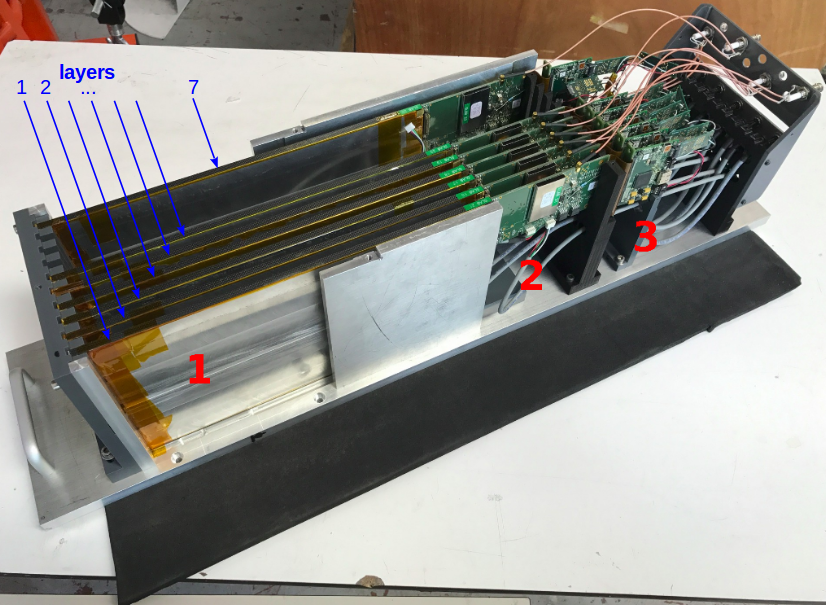
\includegraphics[width=0.65\textwidth]{proto_numbered_2.png} \\
    \caption{}
    \label{proto:a}
  \end{subfigure}%
  \end{tabular}
  \begin{tabular}{l}
    \begin{subfigure}{\textwidth}
    \centering
    %  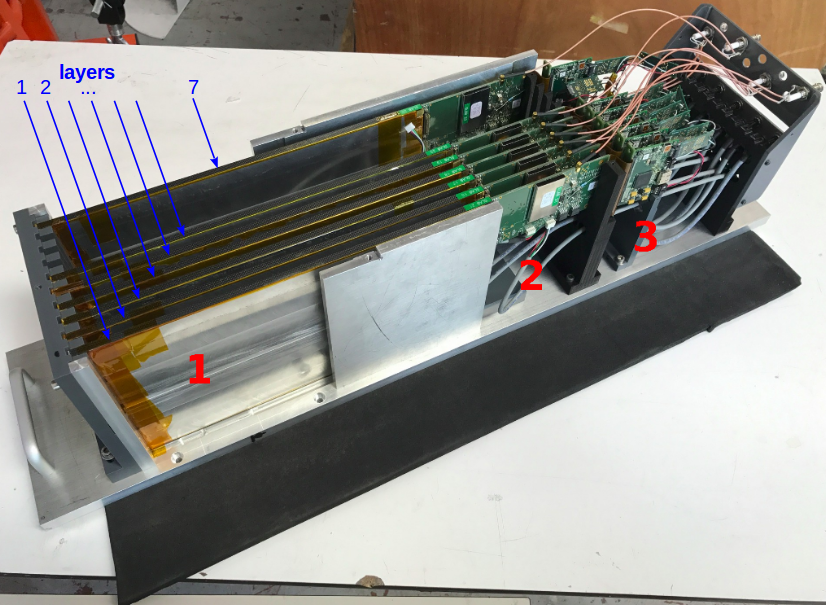
\includegraphics[width=0.65\textwidth]{proto_numbered_2.png} \\
    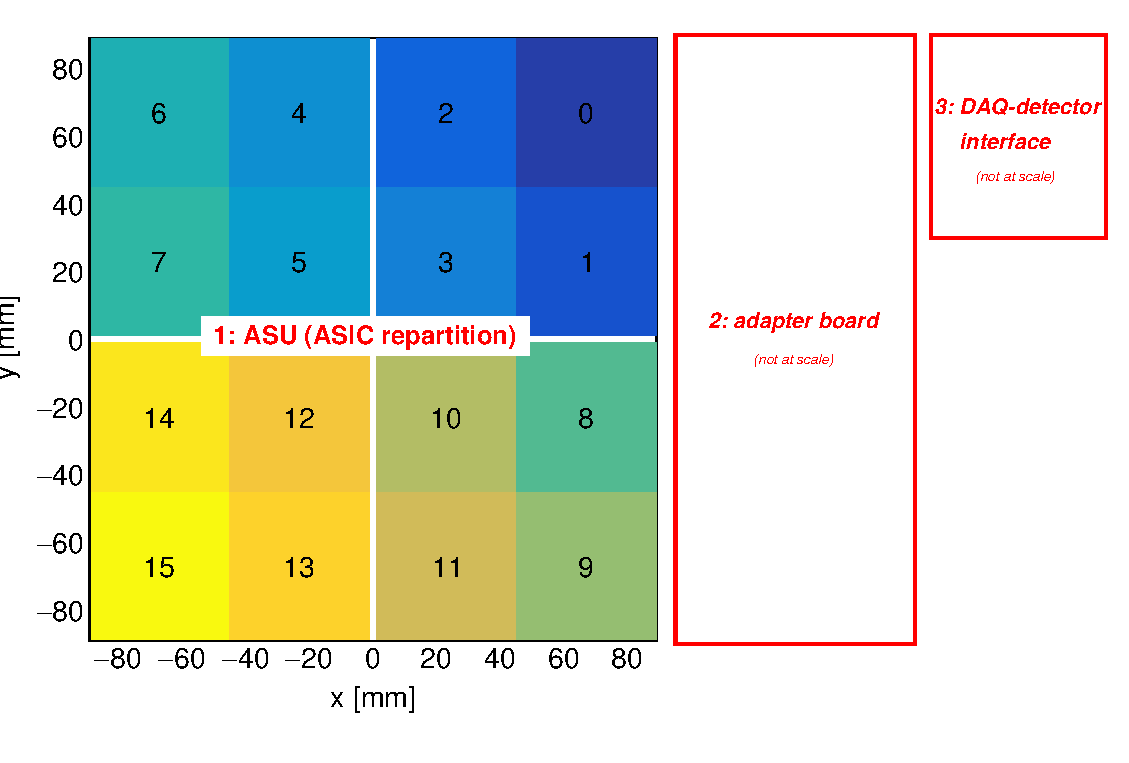
\includegraphics[width=0.75\textwidth]{mapping-eps-converted-to.pdf} \\
    \caption{}
    \label{proto:b}
    \end{subfigure}%
  \end{tabular}
%\begin{tabular}{l}
%  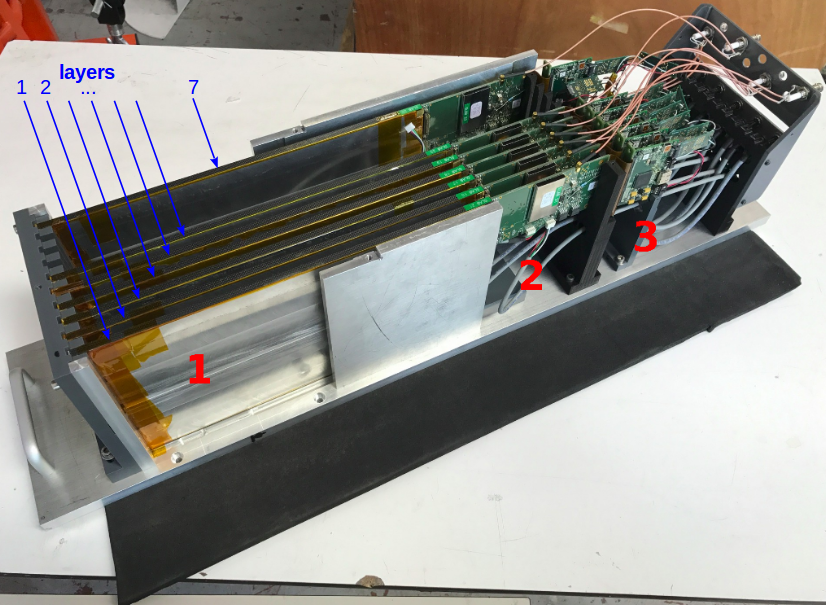
\includegraphics[width=0.65\textwidth]{proto_numbered_2.png} \\
%  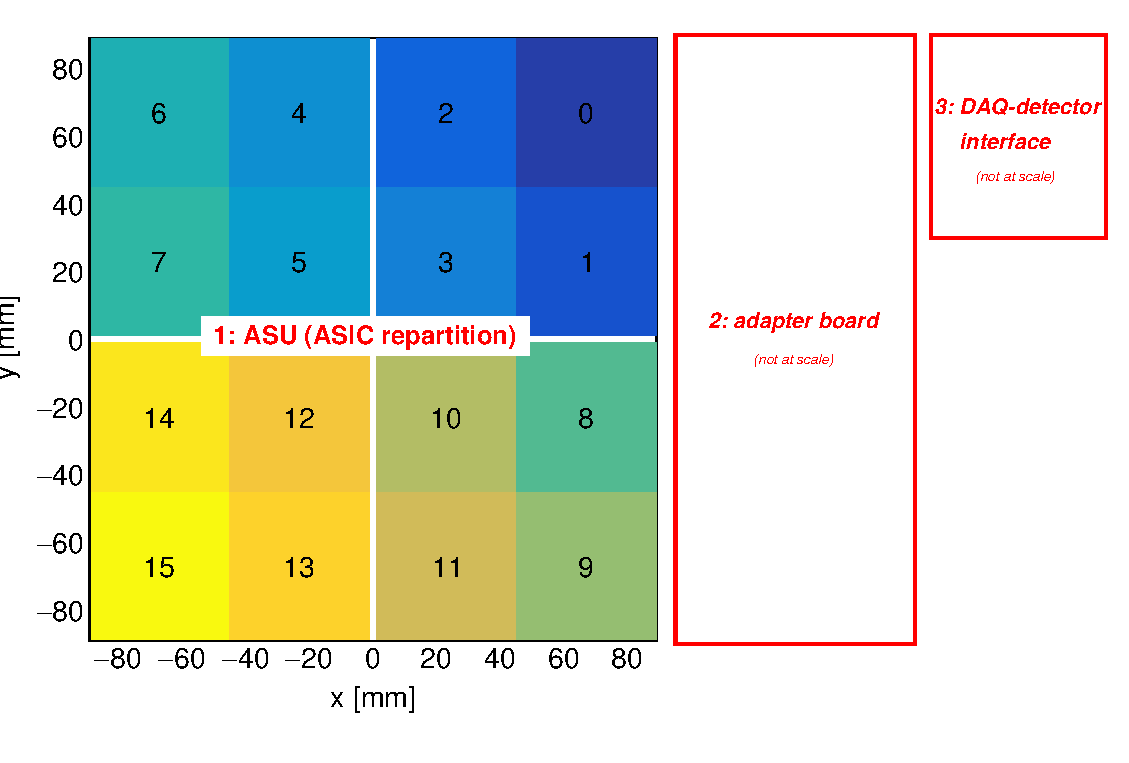
\includegraphics[width=0.75\textwidth]{mapping-eps-converted-to.pdf} \\
%\end{tabular}
\caption{(a) Prototype with 7 layers inside the mechanical housing. (b) Schematic view of the readout modules
  including the surface repartition readout by each ASIC, numbered from 0 to 15. Notice that the adapter board and the DAQ-detector interface drawings are not at scale.}
\label{proto}
\end{figure*}

A picture showing the SiW-ECAL technological prototype setup tested at DESY (Hamburg) in summer
2017 can be seen in Figure \ref{proto:a}.
The setup consists of 7 layers housed in a PVC and aluminium structure that can host up to 10 layers
in slots with a $15-$mm pitch. The first six layers were placed in the first six slots
and the 7th in the last one.
From now on, the layers will be referenced by their numbers from 1 to 7.
The detector was commissioned in the laboratory
and afterwards exposed to a low energy positron beam in the DESY test beam area (line 24) \cite{Diener:2018qap} the first layer located at the most upstream on the beam.
All results presented here are obtained with the detector running in power pulsing mode
and with gated acquisitions of $1-3$ ms at frequencies of 1-5 Hz.

Each layer consists of a readout module
on top of a carbon cradle that protects the sensors
and the sides of the module. The readout module is further wrapped by two aluminium plates
that provide electromagnetic shielding and mechanical stability.
The readout module itself consists of an Active Signal Unit (ASU) and an adapter board
to a data acquisition system (DAQ)\cite{Gastaldi:2014vaa,Rubio-Roy:2017ere,Magniette:2018wdz} at the beginning of the module.
In Figure \ref{proto:a}, the ASUs are covered 
by an aluminium plate as the one marked by the red number 1.
Each ASU consist of a $18\times18$ cm$^2$ sized printed circuit board, PCB,
equipped with 16 VFE ASICs and 4 silicon sensors glued onto the other side.
The PCB features 1024 square pads of $5.5\times5.5$ mm$^2$ that are readout by the ASICs.
Part of the adapter board is also covered by the aluminium plate and the uncovered part 
is seen over the red number 2 in Figure \ref{proto:a}. 
The adapter board also holds other
services e.g. the super capacitance used for the power pulsing. 
This decoupling capacitor of 400 mF with 16 m$\Omega$ of equivalent serial resistance
provides enough local storage 
of power to assure stable low voltage supply during the power pulsing. This capacitor
is seen just above the red number 2 in Figure \ref{proto:a}.
The first component
of the DAQ system, the detector interface board described in \cite{Gastaldi:2014vaa},
is identified in Figure \ref{proto:a} by a red number 3.
For simplicity, the rest of the DAQ system is not shown.  A schematic drawing of a readout module
is shown in Figure \ref{proto:b}.


The VFE ASICs are 16 SKIROC2 \cite{Callier:2011zz,Amjad:2014tha,Suehara:2018mqk}
(Silicon pin Kalorimeter Integrated ReadOut Chip), 
that have been designed for the readout of silicon PIN diodes.
The SKIROC2 in LFBGA package are bump bonded to the PCB.
The version of the ASUs tested in this beam test has a thickness
of 2.8 mm including the ASICs in its current packaging.
Each of these SKIROC2 comprises 64 readout channels
made of a variable-gain preamplifier followed by two branches:
a fast line for the self-trigger decision and a slow line for dual-gain charge measurement.
The gain on the preamplifier is set by changing the feedback capacitor, $C_{f}$.
The fast line consists of a high gain variable CRRC shaper followed by
a low offset discriminator to make the trigger decision.
A common 10-bit DAC provides the threshold of the discriminator.
The slow line is made of a low gain and a high gain CRRC
shapers to handle a large dynamic range.
When a channel triggers, a track and hold cell is used to record the signal at its peaking time
in the dual gain line. The levels of all the others
channels are then also recorded.
% A bandgap ensures the stability with
%respect to supply voltage and temperature for all the requested
%references in the analogue core.
The triggers are timestamped within each gated acquisition with a slow clock
of 5 MHz. The timestamp numbers are called bunch crossing identifiers (BCID).
The charges are stored in the buffers of a switched capacitor array, SCA, and later converted by a 12-bit Wilkinson ADC.
The ASIC consumes, in the power pulsing conditions as foreseen for the ILC, 
27 $\upmu$W per channel.

The four sensors consist of $90\times90$ mm$^{2}$ silicon sensors of
320$\pm15\,\upmu$m thick with high resistivity (larger than 5000 $\Omega\cdot$cm).
Each sensor is subdivided in an array of 256 PIN diodes of $5.5\times5.5$ mm$^2$
connected each to the PCB pads by a dot of conductive glue.
The high voltage to deplete the sensors is delivered to the sensors via a
100 $\upmu$m copper foil isolated from the rest of the setup by a kapton sheet.
It has been estimated that
a MIP traversing the PIN perpendicular to its surface produces, in average,
a signal of 4 fC.


\section{Performance at positron beam test at DESY}
\label{sec:beamtest}

The beam line at DESY provides continuous positron beams in the energy range of 1 to 6 GeV with
rates from a few hundreds of Hz to a few kHz with a maximum of $\sim 3$ kHz for 2-3 GeV. 
In addition, DESY gives access to a bore 1 T solenoid.

The physics program of the beam test can be summarized as follows:

\begin{enumerate}
\item Calibration without tungsten absorber using 3 GeV positrons interacting, in the first approach, as MIPs.
  The beam was normally directed to 81 positions equally distributed over the modules surface.
\item Test in a magnetic field up 1 T using a 3 GeV positron beam.
  For this test, a PVC structure was designed and produced to support one single readout module
  without any tungsten plates.
\item Response to electrons of different energies with a fully equipped detector, {\it i.e}\@. sensitive parts {\it and} tungsten absorber. 
\end{enumerate}

In this paper, we discuss in detail the results of the commissioning of the prototype in Section \ref{sec:commissioning}
and the results of the pedestal, noise and MIP calibration in Section \ref{sec:calib}.
We also show the performance of the single readout tested in a magnetic field in Section \ref{sec:magnetic}. Finally,
a first look to the performance of the detector
in electromagnetic shower events is discussed in Section \ref{sec:showers}.

\subsection{Commissioning of the detector}
\label{sec:commissioning}

Earlier experience with the SKIROC2 ASIC is been reported in \cite{Amjad:2014tha,Balagura:2017pka,Suehara:2018mqk}. 
For the following, the internal SKIROC2 parameters determined in these references are adopted
except if otherwise stated.
Since most of the data taking program consisted of the recording
of MIP level signals, we set a low value of the feedback capacitance of the preamplifier to $C_{f}=1.2$ pF  to obtain
gains of $71.25\,{\rm mV/fC}$ and $7.125\,{\rm mV/fC}$ in the dual-gain charge measurement.
With the higher of both gains, the SKIROC2 ensures a linearity better than 90\% 
for 0.5-200 MIPs, sufficient for
the analysis of electromagnetic showers created by few GeV positrons. All data presented here
were taken with the higher of the two gains.
%Once that the default internal settings of the SKIROC
%are defined, the commissioning was focus on the masking of the noisy channels
%and the optimization of the self-trigger thresholds.

\subsubsection{Masking of noisy readout channels}
\label{sec:noisy}

As a very first step channels are disabled that triggered already at
a threshold above 1 MIP noise runs.
For details the reader is referred to \cite{Bilokin:2018gfn}. The disabled channels can be classified into four categories:


\begin{itemize}
\item Routing issues: The same channels trigger in all layers. This hints at a issue with the routing of the PCB. 
  Following a conservative approach, we added to this set all channels that were noisy in at least three modules.
\item ASIC issues: In case 70\% of the channels of an ASIC triggered at, the entire ASIC was disabled.
  \item Sensor issues: If a wafer showed problems like  e.g. high leakage currents, all channels connected to the wafer were disabled.  
\item Others.
\end{itemize}

\begin{figure}[h!]
  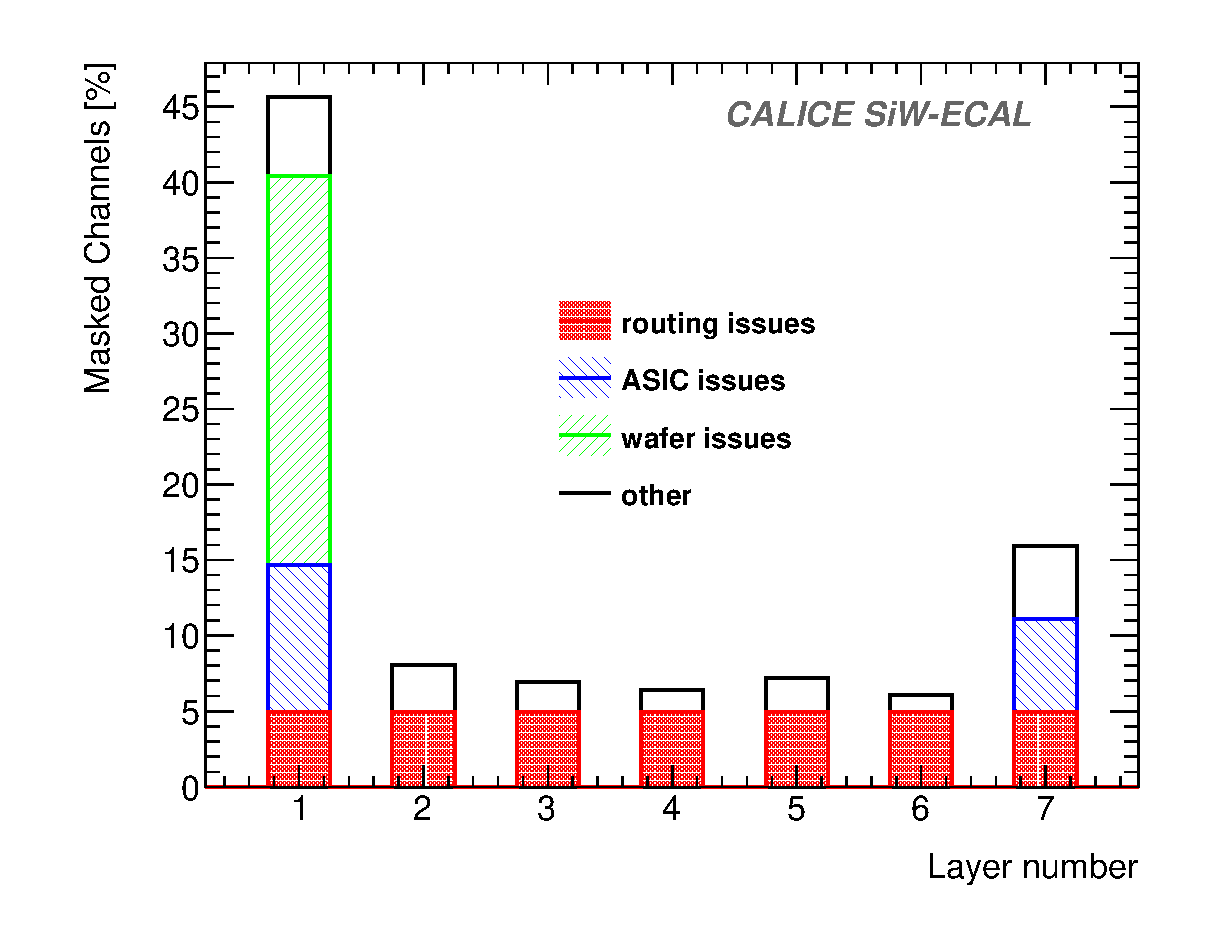
\includegraphics[width=0.5\textwidth]{masked_layer.eps} 
\caption{Fraction of channels with counts above one MIP in noise runs and that have been disabled for the data taking.}
\label{noisycells}
\end{figure}

All these channels have been disabled for the data taking.

\subsubsection{Trigger threshold optimization and signal-over-noise ratio for the trigger}
\label{sec:comm_trigger}

For each ASIC, the threshold of the internal trigger
was optimized by means of dedicated scans of trigger threshold values
with only noise signals or with injected signals of different amplitudes.
The scans start from high values of the thresholds
and this are lowered successively and the number of signals recorded
by each channel are counted. The resulting curves can be approximated by an inverted error function.
A value of the optimal threshold was calculated for every channel by shifting the threshold
from the threshold at the 50\% of the curve plus 3 times the width of the curve, 
with the width defined as half the difference between the thresholds
at which the curve is equal to $50\pm34\%$. The average of the optimal thresholds for all channels
is used as the optimal global threshold to be used by the ASIC.
If the analysis has failed in more than 50\% of the channels ({\it i.e.} because they are masked),
an {\it ad-hoc} high value of the threshold is chosen for the ASIC (250 in DAC units).

Note here that the width of the curve defined before depends on the ratio
of the frequency of the white noise of the electronics and the clock speed of the readout.
Therefore, this quantity is not the optimal estimator of the detector noise.
To achieve this the scan has to be repeated with external signals.
These can either be provided by signals generated by beam particles or by injecting signals into the channels.
Here we follow the second approach. Amplitudes equivalent to 1 and 2 MIPs were injected into channels of an ASIC mounted on a testboard.

The result of these scans is shown in Figure \ref{scurves_injection} for several channels of one SKIROCs.
These curves allow for the trigger threshold calibration and the
estimation of signal-over-noise ratio for the trigger, $(S/N)_{trigger}$, defined as the ratio between the distance of the
1 MIP and 2 MIP threshold curves scans at its 50\% of efficiency and the width of the 1 MIP threshold scan curve.
From the measurement shown in Figure \ref{scurves_injection} we extract a $(S/N)_{trigger}$ ratio of about 12.8.

\begin{figure}[h!t]
    \centering
  \begin{tabular}{l}
	\includegraphics[width=0.5\textwidth]{scurve_pp_fastshaper_ch_DAC_labels.eps}\\ %{scurve_pp_fastshaper_ch_DAC-eps-converted-to.pdf} \\
	\end{tabular}
  \caption{Two sets of threshold curves. Each set consists of theshold curves for individual channels in which a charge is artifially injected using a pulse generator.
    For the set in the left (in blue), an equivalent of 1 MIP was injected. For the set in the right (red), a equivalent of 2 MIPs was injected.
    These curves were obtained in a dedicated testboard \cite{Suehara:2018mqk} to test single SKIROC2 ASICs.}
\label{scurves_injection}
\end{figure}

The trigger threshold calibration (from DAC units to MIPs) is extracted from these curves following a simple formula:

\begin{equation}
	\begin{split}
1 -Threshold[MIP] = \\
\frac{DAC_{50\%}(1\,MIP)-Threshold[DAC]}{DAC_{50\%}(2\,MIP)-DAC_{50\%}(1\,MIP)}
	\end{split}
\end{equation} 

where $DAC_{50\%}(X\,MIP)$ stands for the DAC value in the $50\%$ point of the threshold scan curve obtained with $X$ MIP signals.
This calibration has been applied to all readout modules: see Figure \ref{trigger_thresholds}.
Further dedicated data taking runs with particle beams are needed in the future to measure the uncertainty and spread between SKIROCs and
modules of the used calibration.
%but the first studies using cosmic rays have shown compatible results~\cite{} with the injection tests with 1 MIP signals.

\begin{figure}[h!t]
  \centering
  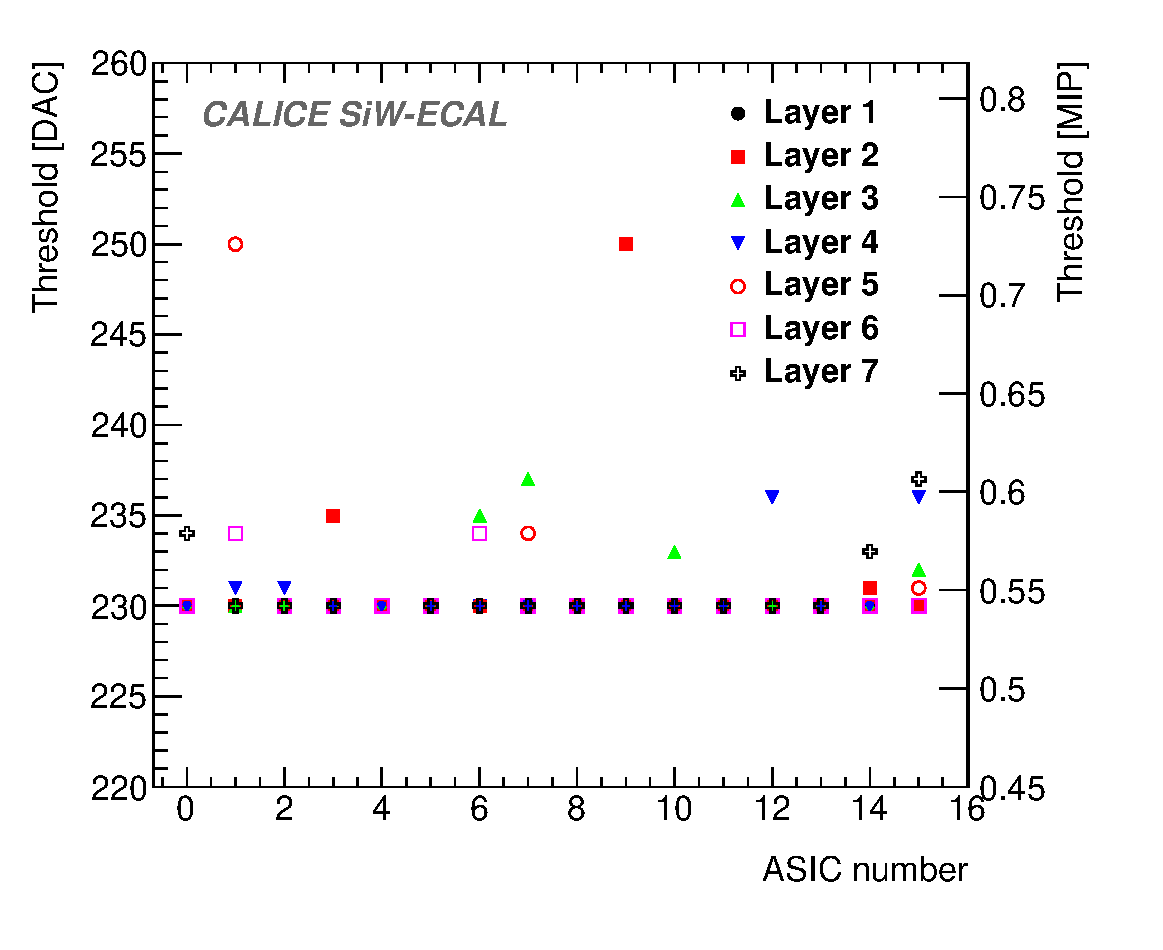
\includegraphics[width=0.5\textwidth]{threshold_chip.eps}
  \caption{Summary of the trigger threshold settings in the internal DAC units and in MIP units.}
\label{trigger_thresholds}
\end{figure}



\subsection{Response to 3 GeV positrons acting as MIPs}
\label{sec:calib}

All the analyses presented here rely on the selection and identification
of tracks-like events. The first step of the reconstruction is the rejection
of two types of fake events due to the ASIC
design: {\it a)} triggers in consecutive BCIDs
due to the preamplifiers sensitivity to instabilities of the power supply; {\it b)}
an artefact of the event validation logical sequence of the ASIC. These fake
events are removed offline using timing information.
Residual electromagnetic showers are rejected by requiring
less than 5 triggers per module.
Tracks are therefore reconstructed by creating clustered
events from the seven layers grouped using their time stamp, allowing for a
tolerance on the BCID of $\pm1$. An event is accepted if at least
three of the layers were clustered together in a track traversing the modules in the
same position
for all modules with a tolerance of $\pm5.5$ {\rm mm} per layer.


\subsubsection{Pedestal and noise determination}
\label{sec:pedestal}

The pedestal distribution for each channel and SCA corresponds to the
distribution of ADC counts recorded by the channel when another one was triggered.
The distributions are fit by a Gaussian. The mean of the Gaussian
is interpreted as the pedestal position. The width of the pedestal is associated to the 
standard deviation of the Gaussian.
Both values are calculated for all ASICS, channels and SCA under test.
Using these calculated pedestal positions, the pedestal subtraction to all measured charges in ADC counts is performed.
This process is done in a layer, ASIC, channel and SCA basis.
As a summary, all the calculated pedestal positions and widths of the ADC for all non-triggered and non-masked
channels and SCAs are shown in Figure \ref{pedestal_all}.
The non-gaussian spread of the pedestal position is explained by the fact that each SCA has its own pedestal value. More important is that the 
width of the distributions is very similar for all
channels and SCAs.
This is a proof of the homogeneity of the noise levels within the system.

\begin{figure}[h!t]
  \centering
  \begin{tabular}{l}
    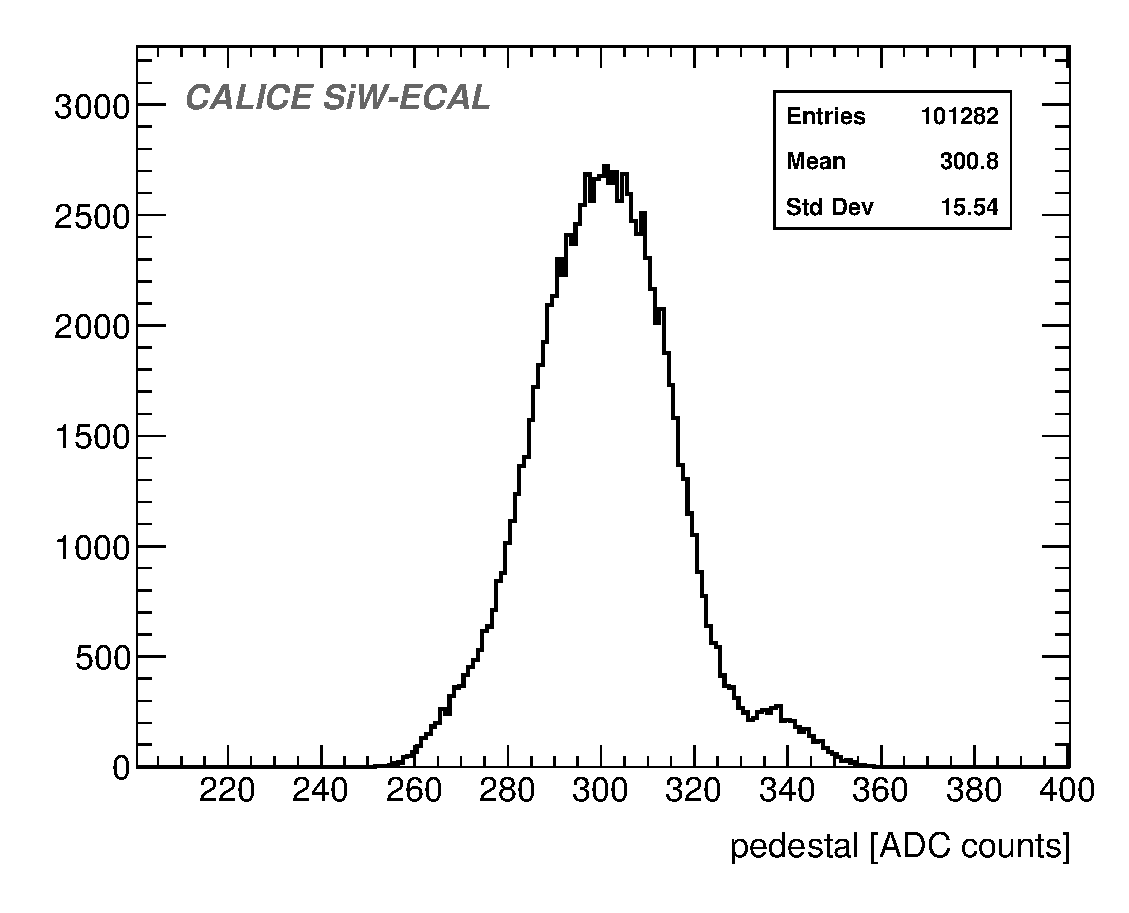
\includegraphics[width=0.5\textwidth]{h_ped_mean_notitle-eps-converted-to.pdf} \\
    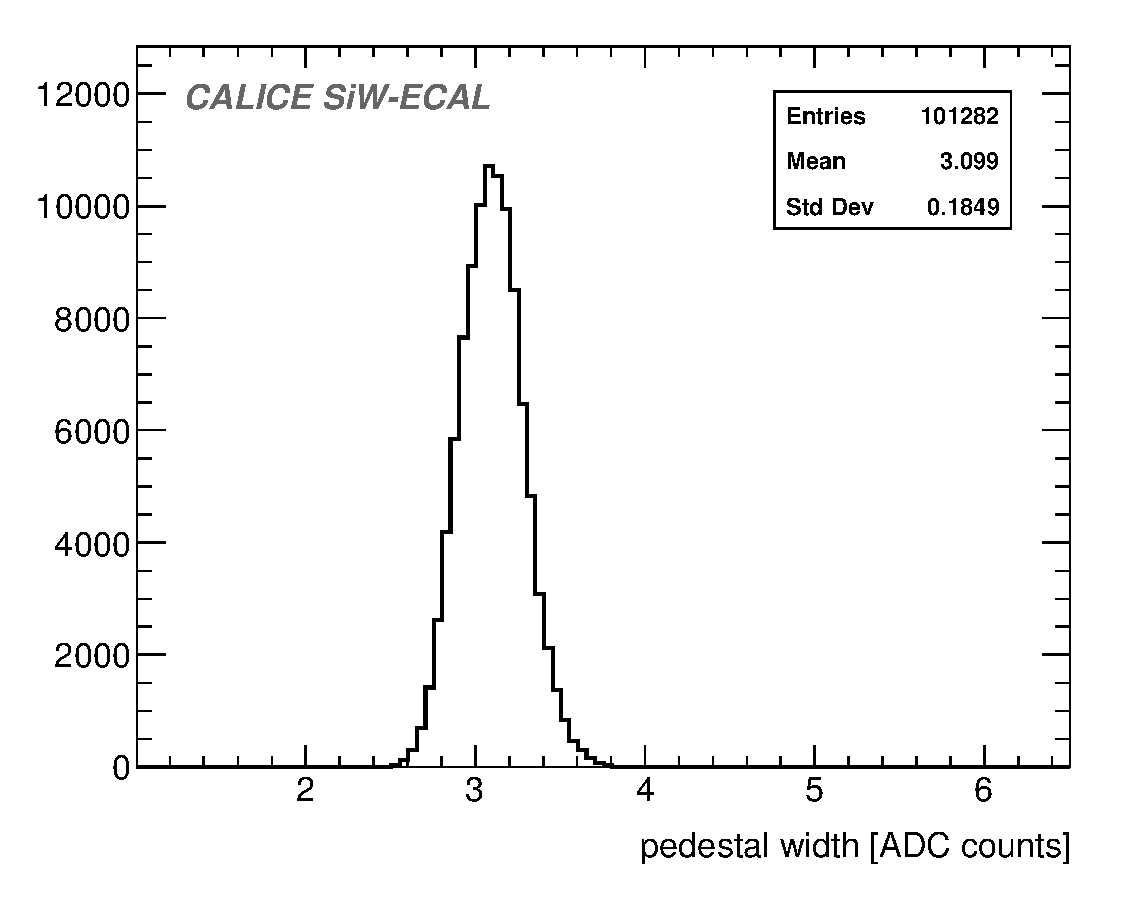
\includegraphics[width=0.5\textwidth]{h_ped_width_notitle-eps-converted-to.pdf}
  \end{tabular}
  \caption{Pedestal mean position (upper) and width (lower) for all channels and all SCAs in the setup.}
\label{pedestal_all}
\end{figure}

\subsubsection{MIP calibration}
\label{sec:mip}

For all channels under test, the resulting charge spectrum of the triggered channels
after pedestal correction are fit by a Landau function convoluted with a Gaussian if the number of events was
larger than 1000. %In the example shown in Figure \ref{signal_pedestal}, this is represented
%by the red curve. In blue it is shown an example of pedestal distribution but only for one SCA
%to make scale of the y-axis reasonable.
The most-probable-value of the Landau function is taken as the MIP value, allowing thus for a direct
conversion from ADC counts to energy in MIP units.

%\begin{figure}[!ht]
%  \centering
%  \begin{tabular}{l}
%    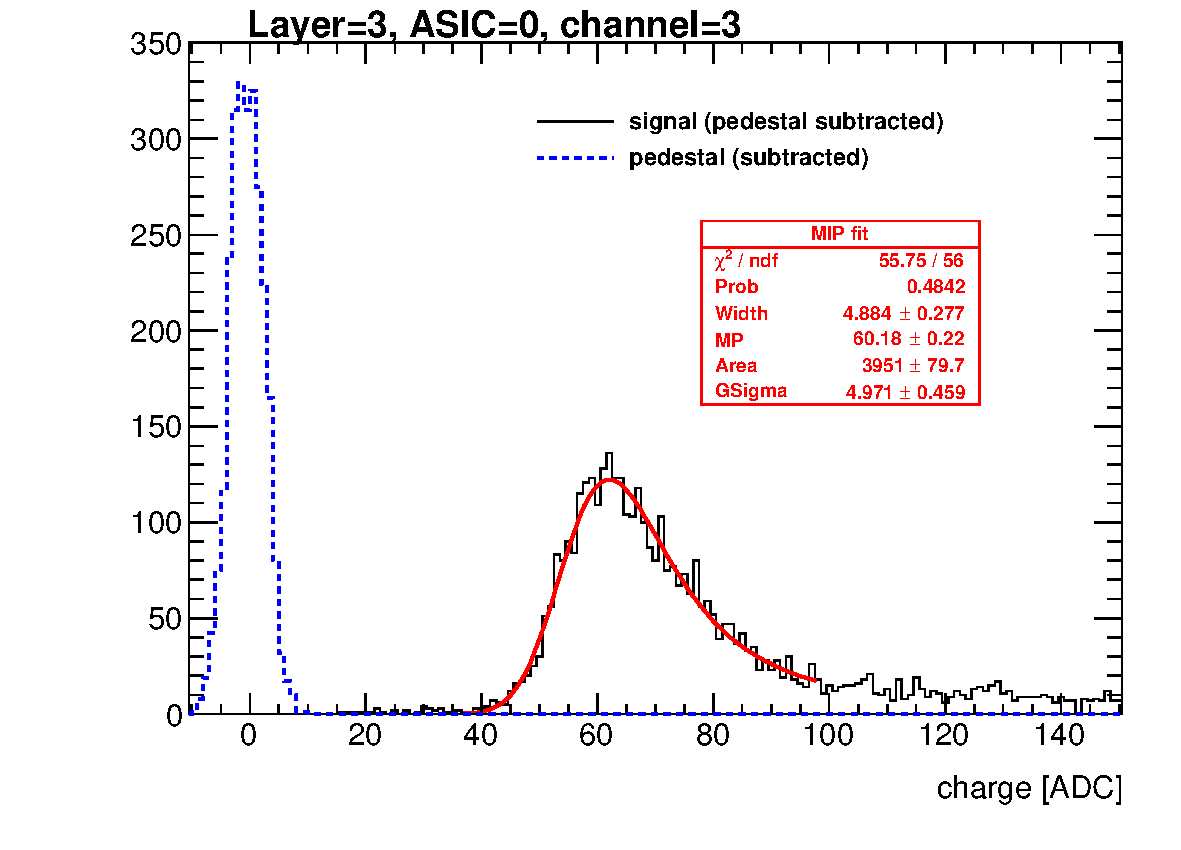
\includegraphics[width=0.45\textwidth]{mip_pedestal_example-eps-converted-to.pdf}
%  \end{tabular}
%  \caption{Representative sample of distributions of the pedestal (blue dashed line) and MIP signal (black continuous line) for one channel.
%    In red, the result of the fit of the MIP distribution.}
%\label{signal_pedestal}
%\end{figure}

The fit succeeded in 98\% of the cases and the spread of the resulting MIP calibration is 5\%.
The remaining channels are discarded in the following analysis. Results are summarized in Figure \ref{mip}.


\begin{figure}[h!t]
  \centering
  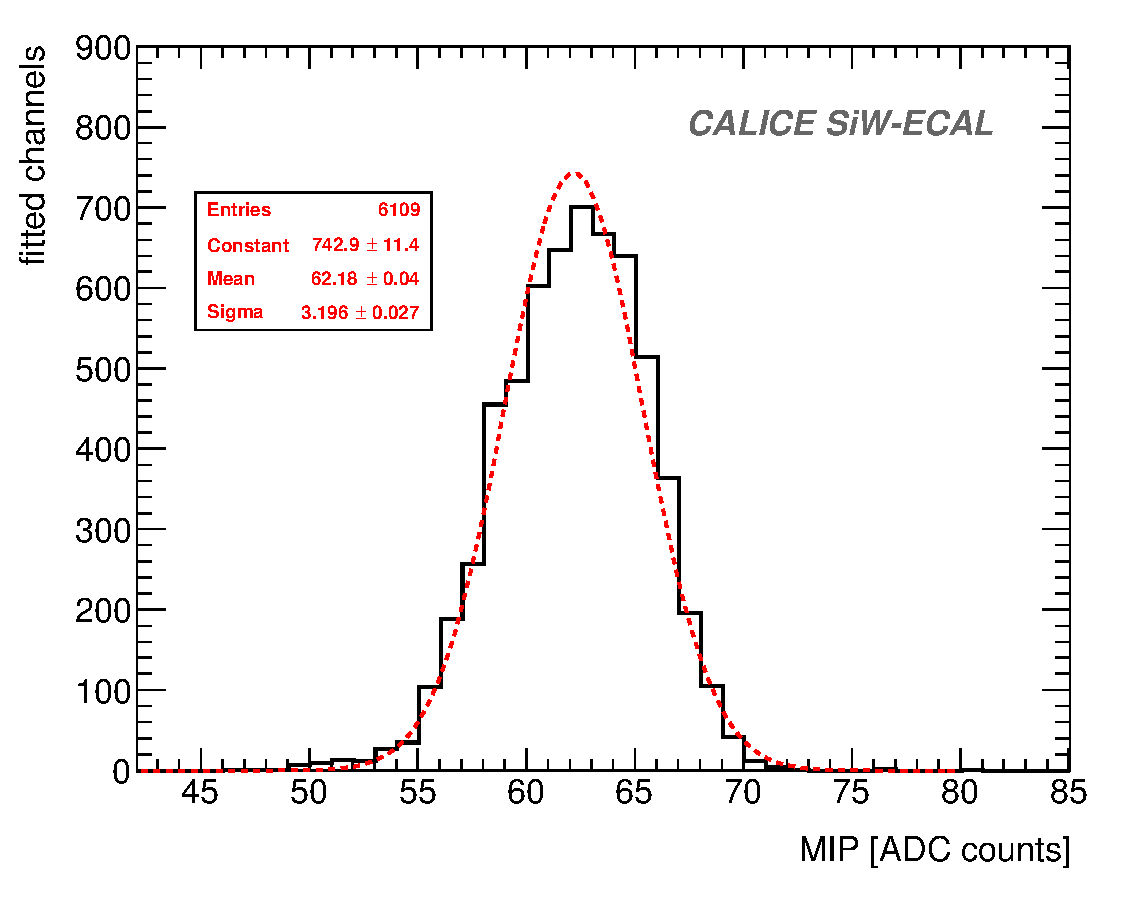
\includegraphics[width=0.5\textwidth]{MIP_summary-eps-converted-to.pdf} \\
\caption{Result of the MIP calibration for all calibrated channels.}
\label{mip}
\end{figure}

\subsubsection{Signal-over-noise ratio for the charge measurement of triggered channels}
\label{sec:sn}

The signal over-noise-ratio for the charge measurement of triggered channels, $(S/N)_{charge}$, is defined 
as the ratio of the calculated MIP values to the noise (the pedestal width) for each channel and SCA.
This quantity has been calculated for all channels under test, giving:
\begin{equation}
(S/N)_{charge}=20.4\pm1.5
\end{equation}

The results are summarized in Figure \ref{mipandSN}.
%The large size of this value allows for a highly efficient offline filtering out of small spurious triggers.
The excellent ratio ensures that low energetic hits just above the trigger threshold can actually be used for the event reconstruction.

\begin{figure}[h!t]
  \centering
  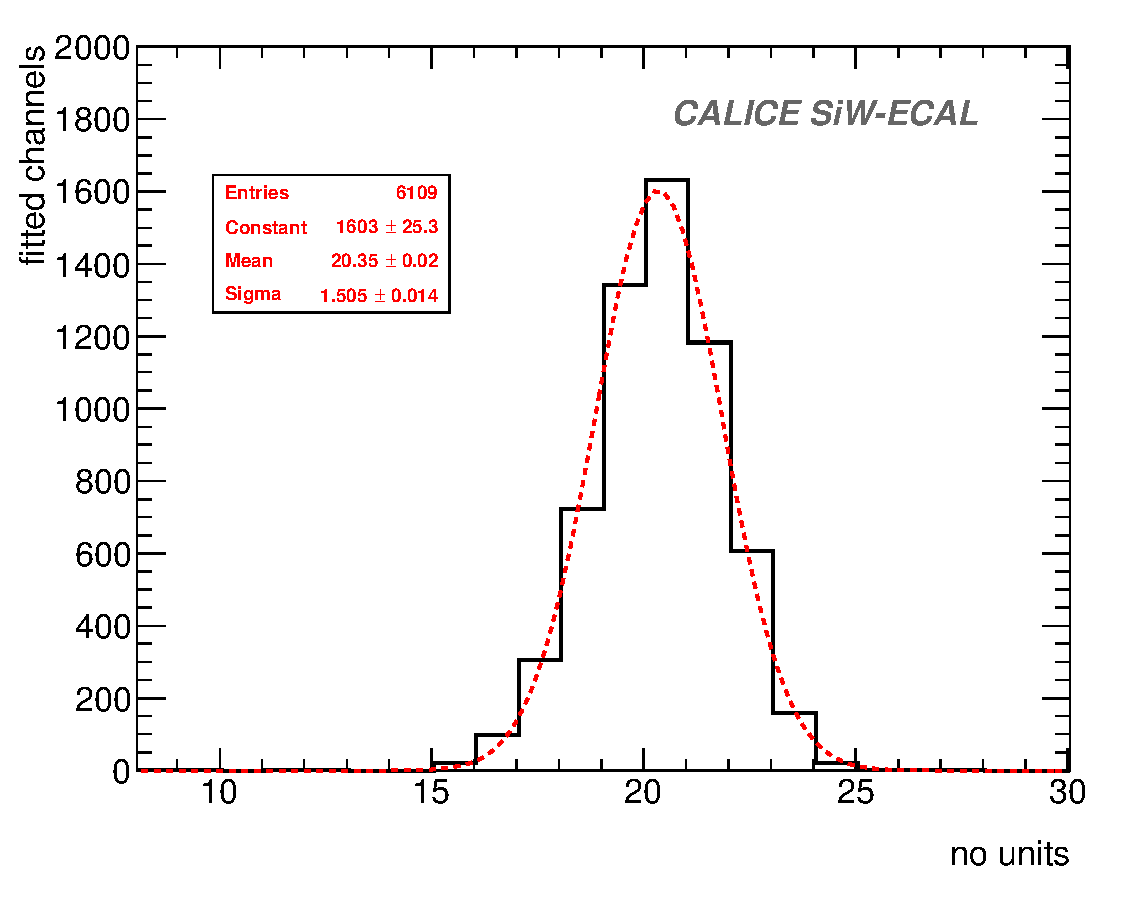
\includegraphics[width=0.5\textwidth]{SN_summary-eps-converted-to.pdf}  
\caption{Distribution of the $(S/N)_{charge}$ for all calibrated channels.}
\label{mipandSN}
\end{figure}

\subsubsection{MIP detection efficiency}
\label{sec:mip}

To evaluate 
the single hit detection efficiency we increased the purity of our tracks sample
by requiring tracks with at least 4 layers with a hit in exactly the same channel.
For the remaining three layers the search region is extended to the eight channels
surrounding the target channel. Residual spurious signals are filtered by requiring a minimal energy deposition of 0.3 MIP.
%Afterwards we 
%check, among the seven layers, which have or not a hit in the same or in eight neighboring channels (if calibrated)
%with energy larger or equal than 0.3 MIP
%to filter out spurious signals.  
%We repeat this procedure for all channels.
The averaged results for every ASIC are shown in Figure \ref{efficiency}.
Except for a few exceptions, the efficiency is 
compatible with $100\%$.
The low efficiencies in the first layer are related to the presence of
noisy channels not spotted during the commissioning. These channels
saturate the DAQ in their ASICs earlier than in others.
In the last layer we also observe few small deviations
which are associated to channels in the periphery, hinting for a small misalignment of the last layer.

\begin{figure}[!t]
  \centering 
  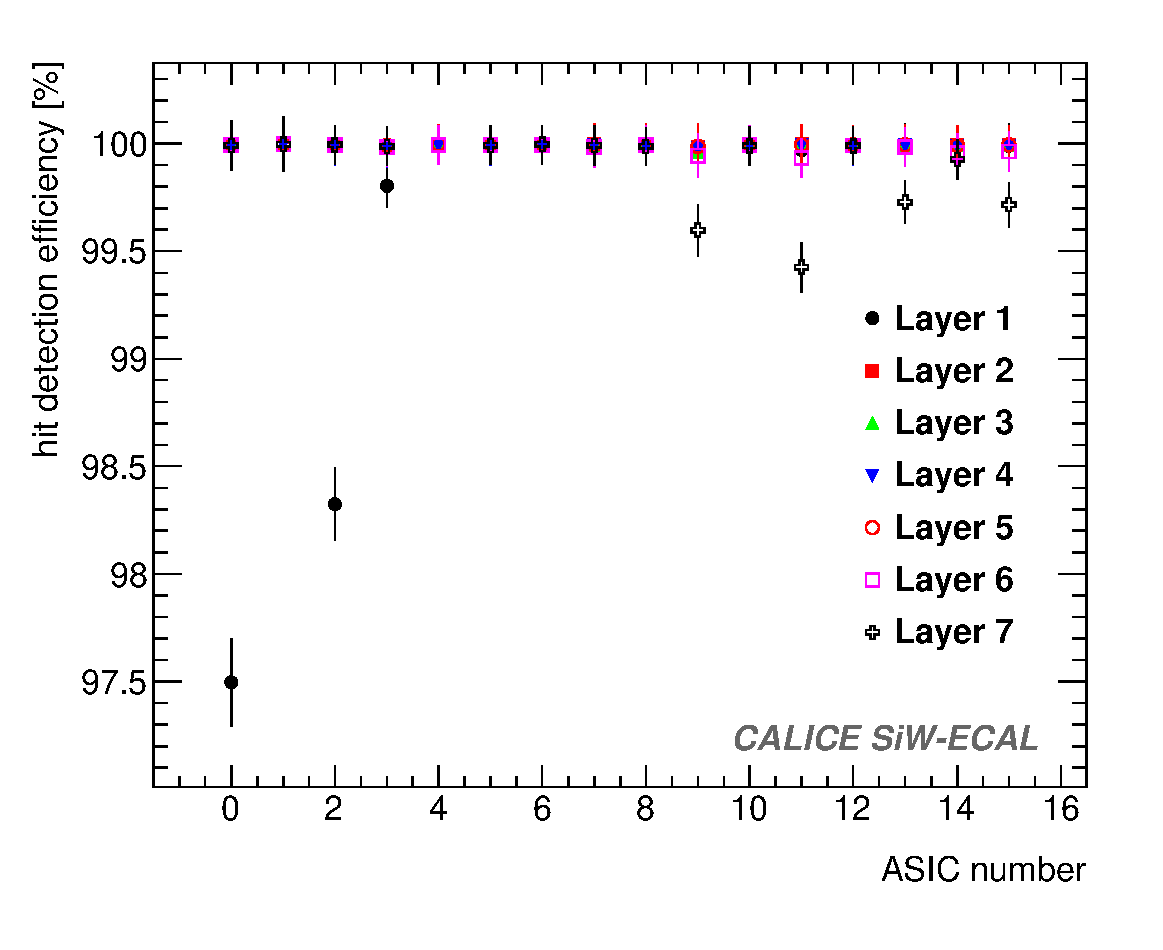
\includegraphics[width=0.5\textwidth]{efficiency_nhits4_chips.eps} \\
  \caption{MIP detection efficiency in high purity samples of tracks of MIP-like acting particles for all layers. The average for all readout channels in each ASICs is shown. The error bars correspond to the standard deviation of the efficiency distribution of all channels in th ASIC.}
\label{efficiency}
\end{figure}


\subsection{Performance of a single readout module in a magnetic field}
\label{sec:magnetic}

The study of the performance of the module inside
inside magnetic fields has been divided in three consecutive steps:
a reference run without magnetic field; a run with a magnetic field of 1 T; a second run with 0.5 T; and a final run without, again, magnetic field.
The beam, 3 GeV positrons, was incident on the area of the PCB readout by the ASIC number 12.
During all this time, the readout module was continuously monitored and did not
show any technical issue or change of performance. Due to the lower beam rates in this area (and the technical character of the test)
we did not collect enough data to present a reliable comparison with the calibration described in the previous sections.
However, we got enough data to study in detail the stability of the pedestal position and width of all channels
in the ASIC 12. Their values are well compatible with the values obtained in Section \ref{sec:calib}.
This is shown in Figure \ref{pedestal_magnetic}.
We see that the agreement is perfect within the statistical uncertainties.
Due to the lower rates in this beam area, the
analysis is only done up to few memory cells.%and at least 500 entries are required in order to calculate the pedestals
%for comparison with the default values.

\begin{figure}[!t]
  \centering
  \begin{tabular}{l}
    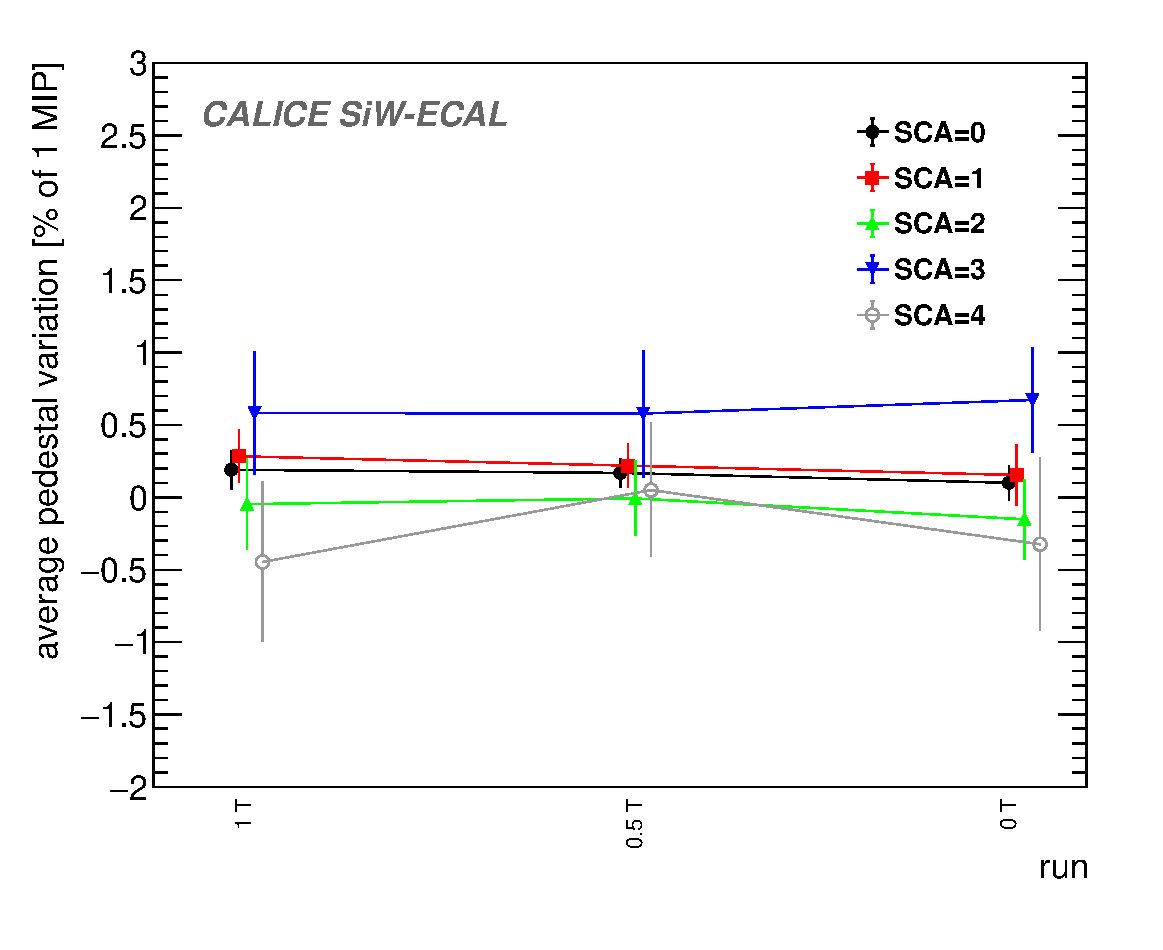
\includegraphics[width=0.5\textwidth]{1T_summary_pedestal.eps} \\
    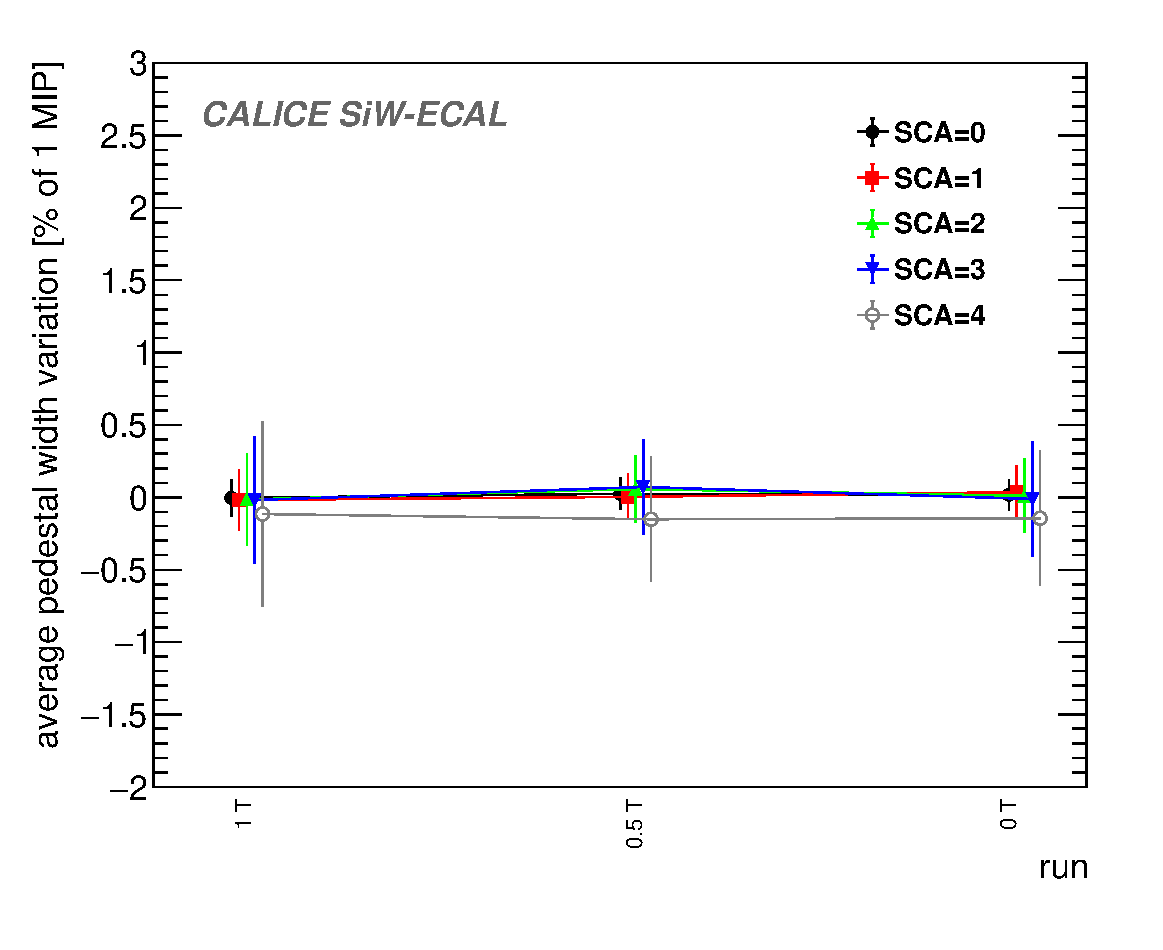
\includegraphics[width=0.5\textwidth]{1T_summary_noise.eps}
  \end{tabular}
  \caption{
    Average deviation of the pedestal mean position (up) and width (down) during the different runs at different magnetic field (1T, 0.5 T and 0T)
    compared with data taken outside of the magnet structure. The error bars correspond to one standard deviation of the averaged values.
    The results for several SCA is presented in each plot, with a slight shift in the $x$-axis to artificially separate the points for better visualization.
  }
\label{pedestal_magnetic}
\end{figure}

\subsection{Performance of the SiW-ECAL for low energy electromagnetic showers.}
\label{sec:showers}
For the last part of the beam test, the stack was equipped with several plates of tungsten of different thickness, interleaved
between the readout modules (including one also between the beam and the first module).
We performed several energy scans of the beam (1, 2, 3, 4, 5 and 5.8 GeV)
and directed it in different positions. In addition, also several distributions of the tungsten absorbers
were put in place. For the analysis of these data we proceed in a similar way than 
the described in Section \ref{sec:mip} for the event building by timestamp. In addition, the single cell calibration described in previous section is applied. In Section \ref{sec:mip}, the events with more than 5 triggers per module were rejected to remove shower like events from the sample, in the present analysis, no constrain on the number of triggers per layer was applied.
The results presented here correspond to the configuration of tungsten amounting 8.4 $X_{0}$ with the beam directed
to the area covered by ASICs number 12-15. For this run, we got enough data to
calculate with high statistics the shower profile for all the energies. This is presented in Figure \ref{showers}.
To calculate the shower profile, we used the the single cell calibration results presented in the previous sections.

\begin{figure}[!t]
  \centering
  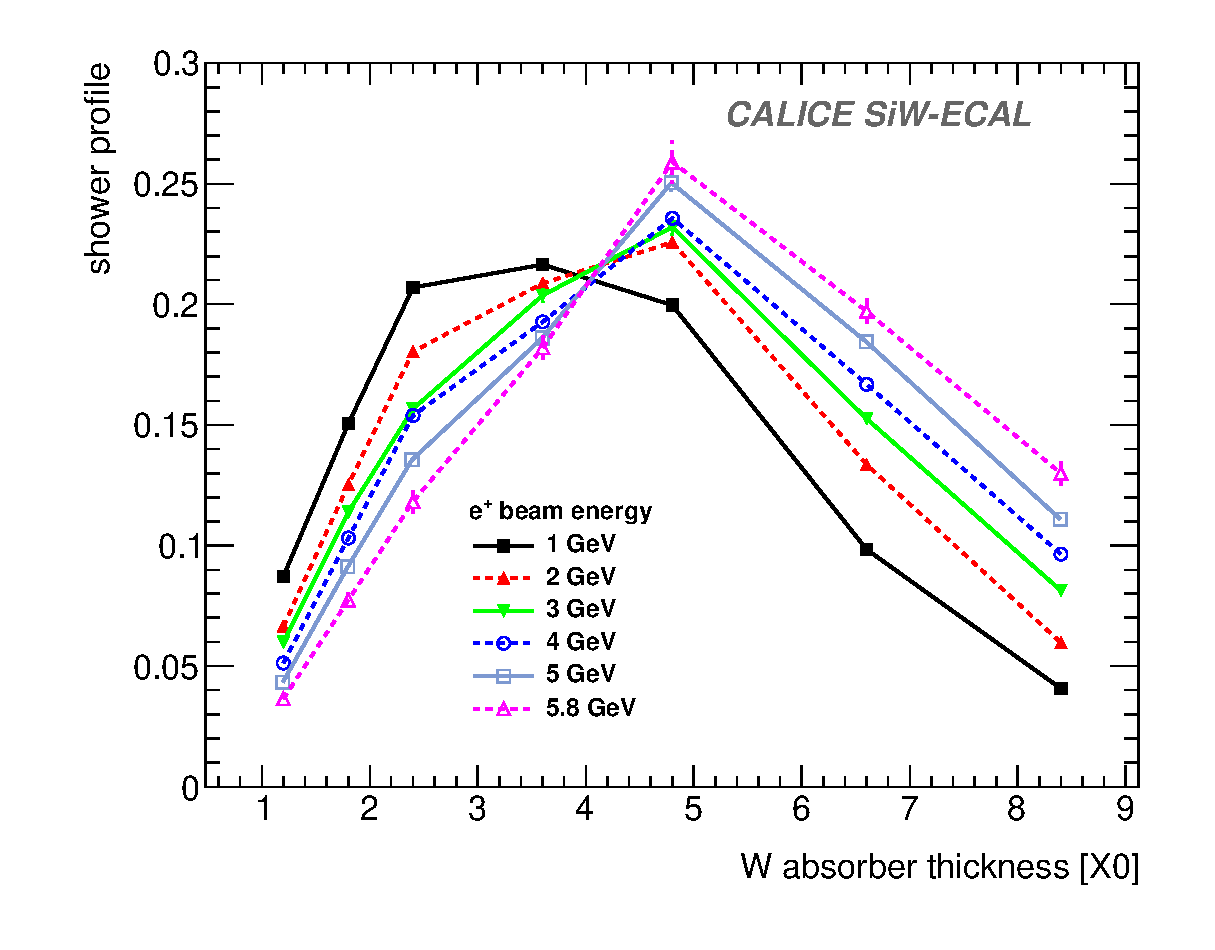
\includegraphics[width=0.5\textwidth]{shower.eps}\\
  \caption{Electromagnetic shower profiles for different beam energies. In the x-axis, we show the accumulated thickness of tungsten absorber in front
    of evert active layer. In the y-axis, the averaged fraction of the total energy measured by every active layer in each electromagnetic shower event. }
\label{showers}
\end{figure}

\section{Summary and outlook}
\label{sec:summary}

In this document we present the results
on the commissioning in beam of a small but fully equipped SiW-ECAL technological prototype
made of readout modules featuring the main characteristics foreseen for future high energy $e^{+}e^{-}$ collider detectors.
%It is the first time that results obtained with data taken by the SiW-ECAL continuosly
%operated in power pulsing are published.
%For the first time results
% SETUP dedicated for physics program with electromagnetic showers.
For the first time results are presented for detection units featuring 1024 channels as
designed for e.g. the ILD Detector in a setup optimized for a physics program dedicated to the study
of electromagnetic showers. The seven layers under study were operated in power pulsed mode.
Therefore this article constitutes a first reference for the detector performance in this operation mode.  
The beam test has allowed for studying in detail 
the performance of the detector.
The detector response is homogeneous with
98\% of the non masked channels calibrated
at a spread of the 5\%.
The signal over noise on the trigger has been evaluated to be about 12.8, a value that allows to
for setting trigger below the MIP level with high efficiency 
although new dedicated beam tests are required to know the uncertainty and spread
of this value 
among different modules and ASICS.
The signal over noise on the charge measurement for triggered channels is 20.4, which 
ensures that all channels with a trigger just about noise level can be used in the data analysis.
The MIP detection efficiency in tracks has been evaluated to be compatible with the 100\% in most of the channels.
This first approach to electromagnetic shower results looks promising although further studies and comparisons with simulations are foreseen
including the data of coming beam tests, which will include further R\&D developments and a potentially larger
stack with up to $\sim20-30$ fully equipped
layers and an homogeneous tungsten absorber distribution amounting up to $\sim24$ $X_{0}$ as foreseen, for example, by the ILD project
for the International Linear Collider.

\section*{Acknowledgments}

This project has received funding from the European Union{\textquotesingle}s Horizon 2020 Research and Innovation program under Grant Agreement no. 654168.
This work was supported by the P2IO LabEx (ANR-10-LABX-0038), excellence project HIGHTEC,
in the framework {\textquotesingle}Investissements d{\textquotesingle}Avenir{\textquotesingle}
(ANR-11-IDEX-0003-01) managed by the French National Research Agency (ANR).
The research leading to these results has received funding from the People Programme (Marie
Curie Actions) of the European Union{\textquotesingle}s Seventh Framework Programme (FP7/2007-2013)
under REA grant agreement, PCOFUND-GA-2013-609102, through the PRESTIGE
programme coordinated by Campus France.
The measurements leading to these results have been performed at the Test Beam Facility at DESY Hamburg (Germany), a member of the Helmholtz Association (HGF).


%\bibliographystyle{JHEP}
\section*{References}
\bibliographystyle{elsarticle-num}
\bibliography{../../references}

\end{document}
